% TODO citation MCM conclusion
% TODO citer le papier de Thibaut
% justifier  le non-MCM
% http://en.wikipedia.org/wiki/Root-raised-cosine_filter
% http://www-users.cs.york.ac.uk/~fisher/mkfilter
% http://www.kwon3d.com/theory/filtering/fil.html
% http://www.winfilter.20m.com/

% matlab/fdatools
\documentclass[twocolumn]{IEEEtran} 
\IEEEoverridecommandlockouts
\title{Hardware LTI Filters Computing Just Right }

\author{\IEEEauthorblockN{Florent de Dinechin, Thibault Hilaire, Matei Istoan\thanks{This work is partly supported by the MetaLibm project (ANR-13-INSE-0007) of the French \emph{Agence Nationale de la Recherche}.}, Benoit Lopez, Abdelbassat Massouri}

\IEEEauthorblockA{
Universit\'e de Lyon, INRIA,  \\
  INSA-Lyon, CITI-INRIA, F-69621, Villeurbanne, France\\
}
}

\usepackage{url}
\usepackage{amsthm,amssymb,amsmath}
\usepackage{xcolor}
\definecolor{light-gray}{gray}{0.6}
\usepackage{graphicx}
\usepackage{multirow}
\usepackage{boxedminipage}
\usepackage{tikz}
\usetikzlibrary{calc} 


\newtheorem{lemma}{Lemma}[section]


% Merci d'utiliser les commandes ci-dessous, comme cela on peut encore changer les notations.
\newcommand{\abserr}{\varepsilon}
\newcommand{\maxerr}{\bound{\abserr}}
\newcommand{\appr}[1]{\widetilde{#1}}
\newcommand{\yout}{\widetilde{y}_{\text{out}}}
%\newcommand{\msbin}{m_{\text{in}}}
\newcommand{\msbin}{1}
\newcommand{\lsbout}{\ell_{\text{out}}}
\newcommand{\msbout}{m_{\text{out}}}
\newcommand{\pin}{\ell_{\text{in}}}
\newcommand{\pbik}[1]{{\pi}_{b_i}(k)}
\newcommand{\paik}[1]{{\pi}_{a_i}(k)}
\newcommand{\epstotal}{\abserr_{\text{out}}}
\newcommand{\maxepstotal}{\maxerr_{\text{out}}}
\newcommand{\epsfinalround}{\abserr_{\text{f}}}
\newcommand{\maxepsfinalround}{\maxerr_{\text{f}}}
\newcommand{\epssopc}{\abserr_{\text{r}}}
\newcommand{\maxepssopc}{\maxerr_{\text{r}}}
\newcommand{\epsytilde}{\abserr_{\text{t}}}
\newcommand{\maxepsytilde}{\maxerr_{\text{t}}}
\newcommand{\bound}[1]{\overline{#1}}
%\newcommand{\wcpg}[1]{||#1||_{\ell^\infty}}
\newcommand{\wcpg}[1]{||#1||}
\newcommand{\wcpgHe}{\wcpg{\mathcal{H}_\abserr}}
%\newcommand{\wcpgHe}{||\mathcal{H}_\abserr||_{\ell^\infty}}






\tikzset{
  x=1ex,y=1ex,
  hwblock/.style={draw, rectangle, rounded corners=.3, very thick, fill=black!5, font=\sf, minimum height=5ex},
  hwbus/.style={very thick,>=stealth},
  hwwire/.style={thin, >=stealth, },
  hwword/.style={draw, rectangle, minimum height=3ex},
  bitwidth/.style={font=\scriptsize,midway,right}
}


\graphicspath{{Figures/}}

\begin{document}
\maketitle
\begin{abstract}
Linear Time Invariant (LTI) filters are often specified and simulated using high-precision software, before being implemented in low-precision hardware. 
A problem is that the hardware does not behave exactly as the simulation due to quantization and rounding issues.
This article advocates the construction of LTI architectures that behave as if the computation was performed with infinite accuracy, then rounded only once to the low-precision output format.
From this minimalist specification, it is possible to deduce the optimal values of many architectural parameters, including all the internal data formats. 
This requires a detailed error analysis that captures the rounding errors, but also their infinite accumulation in infinite impulse response filters.
This error analysis may then guides the design of hardware satisfying the accuracy specification at the minimal hardware cost. 
This is illustrated on the case of low-precision LTI filters implemented in FPGA logic.
This approach is fully automated in a generic, open-source architecture generator tool built upon the FloPoCo framework, and  evaluated on a range of  Finite and Infinite Impulse Response filters. 
\end{abstract}
%  specification enables a very simple and high-level interface.

% \begin{IEEEkeywords}
% \end{IEEEkeywords}

\section{Introduction}

This article addresses the automatic implementation of Linear Time Invariant (LTI) digital filters. 
Such filters are ubiquitous in signal processing and control, and are typically defined as a transfer function in the frequency domain:
\begin{equation}
  \label{eq:firsteq}
  \mathcal{H}(z)=\frac{\sum_{i=0}^{n}b_iz^{-i}}{1+\sum_{i=1}^{n}a_iz^{-i}}  \quad \forall z \in \mathcal{C}.
\end{equation}
Equivalently, the output signal $y(k)$ and the input signal $u(k)$ may also be related by the following equation:
\begin{equation}
  \label{eq:ideal-filter}
  y(k) = \sum_{i=0}^{n}b_iu(k-i) - \sum_{i=1}^{n}a_iy(k-i)
\end{equation}



Equation (\ref{eq:firsteq}) or (\ref{eq:ideal-filter}), along with a mathematical definition of each coefficient $a_i$ and $b_i$, constitute the \emph{mathematical specification} of the problem.
In this specification, the coefficients are considered as real numbers. 
They may even be given as explicit formulae, as for instance in textbook pulse-shaping filters (half-sine or root-raised cosine) used in wireless communication \cite{ZigBeeStandard}. 
However, the coefficients may also be provided as high-precision floating-point numbers.


This article deals with the \emph{implementation} of such a specification as fixed-point hardware operating on low-precision data (typically 8 to 24 bits).

To specify such an {implementation}, a designer needs to define several parameters on top of the mathematical specification.
Obviously, he needs to define the finite-precision input and output formats. 
He also needs to make several architecture choices, some of which will impact the accuracy of the computation. 
For instance, each real-valued coefficient must be rounded to some internal machine format.
A naive choice is to round the coefficients to the input/output format, but then for large values of $n$ (the filter order), the result can become very inaccurate.
Some design tools for filter synthesis let the designer chose an extended internal precision. 
The risk is then to obtain an architecture that wastes area, time and power by computing more accuracy than it can output.

The main contribution of this article is to show that such design decisions can be automated,  based on  the following simple claim:

\emph{An LTI architecture should be designed to compute results that are accurate to the last bit, but no more}.

This claim is based on two common-sense observations.
On the one hand, there is no point in designing an architecture that outputs  bits which we know hold no useful information. 
% (this would mean a waste of wires and a waste of power, not only on these wires, but also on subsequent operators that will perform computations on these noisy bits).
On the other hand, there is no point in computing internally to an accuracy that we will not be able to express on the output.

\begin{figure}
  \centering
  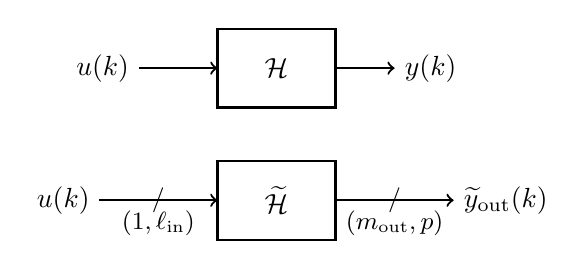
\begin{tikzpicture}[x=1cm,y=1cm]
    \draw (-2,0.5) rectangle ++(1.5,1)[thick] node [midway]{$\mathcal{H}$}; 
    \draw (-3, 1) node [left]{$u(k)$} -- (-2,1) [->, thick] ; 
    \draw (-0.5, 1) -- ++(0.75,0) [->, thick] node[right]{$y(k)$}; 

    \draw (-2+0,0.5-1.678) rectangle ++(1.5,1)[thick] node [midway]{$\widetilde{\mathcal{H}}$}; 
    \draw (-3.5+0, 1-1.678)node [left]{$u(k)$}  -- (-2+0,1-1.678) [->, thick] node[midway] {\small /} node[below, midway] {\small$(\msbin,\pin)$}; 
    \draw (-0.5+0, 1-1.678) -- ++(1.5,0) [->, thick] node[right]{$\yout(k)$}  node[midway] {\small /} node[below, midway] {\small$(\msbout,p)$}; 
  \end{tikzpicture}

\caption{The ideal filter (top) and its implementation (bottom) \label{fig:ltiideal}}
\end{figure}


\begin{figure}
  \centering
    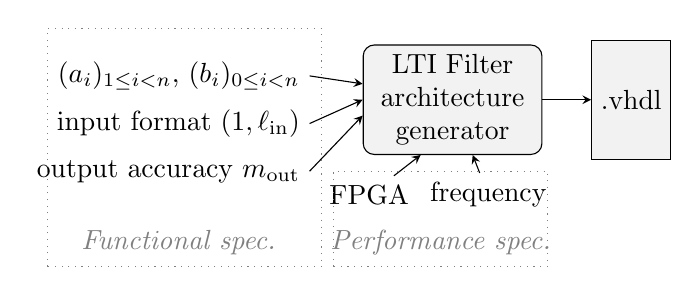
\begin{tikzpicture}
      \node[draw,align=center,fill=black!5,rounded corners, minimum width=15ex, minimum height=5ex] (flopoco) at (0,2ex) {LTI Filter\\architecture\\generator};
      \node[left] (ai)      at (-12ex,4ex)  {$(a_i)_{1\le i < n}$, $(b_i)_{0\le i < n}$};   
      \node[left] (precx)   at (-12ex,0ex) {input format $(\msbin, \pin)$};   
      \node[left] (precy)   at (-12ex,-4ex) {output accuracy $\msbout$};   
      \node[] (target)  at (-7ex,-6ex) {FPGA};   
      \node[] (freq)    at (3ex,-6ex)  {frequency};   
      \node[draw, rectangle,fill=black!5, minimum height=10ex] (vhdl) at (15ex,2ex) {.vhdl};   
      \draw[->,>=stealth] (ai.east) -- (flopoco.170) ;
      \draw[->,>=stealth] (precx.east) -- (flopoco.180) ;
      \draw[->,>=stealth] (precy.east) -- (flopoco.190) ;
      \draw[->,>=stealth] (target) -- (flopoco.240) ; 
      \draw[->,>=stealth] (freq) -- (flopoco.290) ;
      \draw[->,>=stealth] (flopoco.east) -- (vhdl.west) ;

      \draw[dotted,black!50] (-34ex,-12ex) rectangle +(23ex,20ex);   
      \node[black!50]  at (-23ex,-10ex) {\emph{Functional spec.}};   
      \draw[dotted,black!50] (-10ex,-12ex) rectangle +(18ex,8ex);   
      \node[black!50]  at (-1ex,-10ex) {\emph{Performance spec.}};   
  \end{tikzpicture}
  \caption{Interface to the proposed tool. 
    The coefficients $a_i$ and $b_i$ are considered as real numbers: 
    they may be provided as high-precision numbers from e.g. Matlab, or even as  mathematical formulae such as \texttt{sin(3*pi/8)}.
    The integers $m$, $l$ and  $p$  respectively denote the bit weights of the most significant and least significant bits of the input, and the least significant bit of the result.
  In the proposed approach, $p$ specifies  output precision, but also  output accuracy.}
  \label{fig:interface}
\end{figure}

Section \ref{sec:erroranalysisLTI} will show how this claim may be formalized and developed into a complete error analysis.
This enables a very simple interface (Fig.~\ref{fig:interface}) to an LTI implementation tool. 
The designer may  focus on those  design parameters which are relevant: the (real) coefficients, and the input/output formats. 
% It will be shown that thethe optimal internal format to which coefficients will be rounded may be computed, and therefore neednot be a concern to a designer.
The construction of a minimal-cost architecture of proven last-bit accuracy can be fully automated out of this information.


As an illustration, an open-source tool demonstrates this implementation process for a particular hardware target: FPGAs based on Look-Up Tables (LUTs).
Built upon the FloPoCo  project\footnote{\url{http://flopoco.gforge.inria.fr/}}, this tool automatically generates VHDL  for LTI filters from the specification of Fig.~\ref{fig:interface}. 
It also benefits from the FloPoCo back-end framework: the generated architectures are optimized for a user-specified FPGA family, and a user-specified frequency (Fig.~\ref{fig:interface}). 


This demonstrator also incorporates several architectural novelties.
The constant multipliers are built using an evolution of the KCM algorithm \cite{Chapman93:edn,Wirthlin2004} that manages multiplications by a real constant without needing to truncate it first \cite{DinechinTakeugmingTanguy2010}.
The summation is efficiently performed thanks to the BitHeap framework recently introduced in FloPoCo \cite{DinIstSer2013-FPL-BitHeap}.
These technical choices lead to logic-only architectures suited even to low-end FPGAs, a choice motivated by work on implementing the ZigBee protocol standard \cite{ZigBeeStandard}
(some of the examples illustrating this article address this standard).
However, the same philosophy could be used to build other architecture generators, for instance exploiting embedded multipliers and DSP blocks.

TODO meilleur expos\'e du plan quand il aura converg\'e.




\section{Definitions and notations}
\label{sec:definitions}



\subsection{Fixed-point formats}
There are many standards for representing fixed-point data. 
The one we use in this work is inspired by the VHDL \texttt{sfixed} standard.
For simplicity we only deal with signed fixed-point number, classically represented in two's complement.
A fixed-point format is then fully specified by two integers $(m,p)$ that respectively denote the position of the most significant and least significant bit (MSB and LSB) of the data.
The respective values of the MSB and LSB are thus $2^m$ and $2^p$.
Sometimes we will call the LSB position $p$ the \emph{precision} of the format. 
The MSB position denotes its \emph{range}.
Both $m$ or $p$ can be negative if the format includes fractional bits.
Besides, $m$ is also the position of the sign bit. 
As both MSB and LSB are included, the size of a fixed-point number is $m-p+1$.
For instance, for a signed fixed-point format representing numbers  in $(-1,1)$ on 16-bit, we have one sign bit to the left of the point and 15 bits to the right, so $(m,p)=(0,-15)$.  

In all the following, we note $p$ (without a subscript) the precision of the output format, such that $2^{p}$ is the weight of the least significant bit (LSB) of $\yout$.

\subsection{Approximations and errors}

The overall error, noted $\epstotal$, of an architecture that outputs a fixed-point result $\yout$ is defined as the difference between the computed value  and its mathematical specification, noted $y$:
\begin{equation}
  \label{eq:globalerror1}
  \epstotal\quad  =\quad   \yout-y
\end{equation}

More generally, in all the article, we denote $\abserr$ (with some subscript) an error, which is always defined as the difference between a more accurate term and a less accurate one.

We also try to use tilded letters (e.g. $\yout$ above) for approximate or rounded terms.
This is but a convention, and the choice is not always obvious.
For instance, the $u(k)$  in (\ref{eq:ideal-filter}) are fixed-point inputs, and most certainly the result of some approximate measurement or computation.
However, from the point of view of the architecture, inputs are given, so they are considered exact.

In all the following, we also note  $\maxerr$ a bound on $\abserr$, \emph{i.e.} the maximum value of $|\abserr|$.


\subsection{Perfect and faithful rounding}
The rounding of a real such as our ideal output $y$ to the nearest fixed-point number of precision $p$ is denoted  $\circ_{p}(y)$.
In the worst case, it entails an error  \mbox{$|\circ_{p}(y)-y| < 2^{p-1}$}. 
For instance, rounding a real to the nearest integer ($p=0$) may entail an error up to  $0.5=2^{-1}$.
This is a limitation of the format itself.
Therefore, the best we can do, when implementing (\ref{eq:ideal-filter}) with a precision-$p$ output, is a \emph{perfectly rounded} computation with an error bound $\maxepstotal=2^{p-1}$.


Unfortunately, reaching perfect rounding accuracy may require arbitrary intermediate precision. 
This is not acceptable in an architecture. 
We therefore impose a slightly relaxed constraint:  $\maxepstotal<2^{p}$.
We call this \emph{last-bit accuracy}, because the error must be smaller than the value of the last (LSB) bit of the result.
It is sometimes called \emph{faithful rounding} in the literature.

Considering that the output format implies that $\maxepstotal\ge 2^{p-1}$, it is still a tight specification. 
For instance, if the exact $y$ happens to be a representable precision-$p$ number, then a last-bit accurate architecture will return exactly this value.
%Also, increasing $p$ by one divides $\overline{\abserr}$ by two.

The main reason for chosing last-bit accuracy over perfect rounding is that, as will be shown in the sequel, it can be reached with very limited hardware overhead.
Therefore, in terms of cost and efficiency, an architecture that is last-bit-accurate to $p$ bits makes more sense than a perfectly rounded architecture to $p-1$ bits, for the same accuracy bound $2^{p}$.

In any case, the main conclusion of this discussion is the following: specifying the output precision ($p$ on Fig.~\ref{fig:interface} is enough to also specify the accuracy of the implementation.


% \subsection{Tool interface}

% To sum up, the ideal interface (Fig.~\ref{fig:interface})  should
% \begin{itemize}
% \item   allow a
%   user to input the $(a_i)_{0\le i < N}$ to the tool either as
%   mathematical formulas, or as arbitrary-precision floating-point
%   numbers.  Our current implementation only supports the latter so
%   far;

% \item offer one single integer parameter $p$, to serve both as accuracy specification and as the definition of the LSB of the output format.
% \end{itemize}

%Let us now show that the MSB of the output format, as well as all the internal precision parameters, may be deduced from the parameters depicted on Fig.~\ref{fig:interface}. 

% She should not have to convert the $a_i$  to some fixed-point format, nor have to select the format of intermediate computations. 
% We show in this article that optimal decisions can be made for these choices, and that they don't even involve heuristic.
% This is a direct consequence of the specification of the operator as last-bit-accurate.

\subsection{Worst-case peak gain of an LTI filter}
\label{sec:WCPG-def}
The following lemma captures the amplification of a signal by an LTI filter.
\begin{lemma} \label{lemma:wcpg}
If the input  $u(k)$ to an LTI filter $\mathcal{H}$ is bounded by $\bound{u}$ (\emph{i.e.} $\forall k \quad |u(k)|\leq \bound{u}$), then the output $y(k)$ will be bounded iff the moduli of the poles of the transfer function $\mathcal{H}(z)$ are all strictly smaller than 1. This property is know as the Bounded Input Bounded Output (BIBO) stability \cite{Kail80}.

In this case, the Worst-Case Peak Gain (WCPG) $\wcpg{\mathcal{H}}$ of the filter $\mathcal{H}$ is defined as the largest possible peak value of the output $y(k)$ over all the possible bounded input $u(k)$:
\begin{equation}
	\bound{y} = \wcpg{\mathcal{H}} \bound{u} \ .
\end{equation}
The WCPG  
%can be seen as a $\ell^{\infty}/\ell^{\infty}$ induced norm, and 
can be computed as the $\ell_1$-norm of the impulse response $h(k)$ of $\mathcal{H}$, \emph{i.e.} $\wcpg{\mathcal{H}}=\sum_{k=0}^{\infty}|h(k)|$.
\end{lemma}

\begin{proof}
	Due to the linearity of the filter $\mathcal{H}$ and the property of the impulse response, the output $y(k)$ is a convolution between the impulse response and the input:
	\begin{equation}\label{eq:bound_y}
 		y(k) = \sum_{l=0}^{k} h(l) u(k-l)
	\end{equation}
	So
	\begin{equation}
 		|y(k)| \leq \sum_{l=0}^{k} |h(l)| \bound{u}
	\end{equation}
	with equality if $\forall 0 \leq l \leq k \quad u(k-l)=\text{sign}(h(l))\bound{u} $.
	% Commented by F2D ??? Then the bound $\bound{y}$ is deduced with eq. \eqref{eq:bound_y}
\end{proof}


The bound $\bound{y}$ is quite conservative in practice. 
However, it is always possible to exhibit an input $u(k)$ bounded by $\bound{u}$ such that the corresponding output is arbitrary close to its bound $\wcpg{\mathcal{H}} \bound{u}$. 

The value of the Worst-Case Peak Gain  can be computed at any arbitrary precision~\cite{Volk15a}.











\section{Sum of products computing just right\label{sec:SoPC}}

In this section, we address the sub-problem of building a Sum of Product by Constants (SOPC) architecture, \emph{i.e.} an architecture computing 
\begin{equation}
  \label{eq:sopc0}
  y=\sum_{i=1}^{n}c_ix_i
\end{equation}
for a set of real constants $c_i$, and a set of fixed-point inputs $x_i$, each with its fixed-point format $(m_i,\ell_i)$.
The interface to this problem is shown on Figure~\ref{fig:interfaceSOPC}.
In the context of an LTI filter (illustrated by Figure~\ref{fig:ltiarch}), the $c_i$ may be $a_i$ or $b_i$, and the $x_i$ may be either some delayed $u_i$, or some delayed $y_i$.
The format of the $y_i$ is, in general, different from that of the $u_i$. 

\begin{figure}[h]
  \centering
    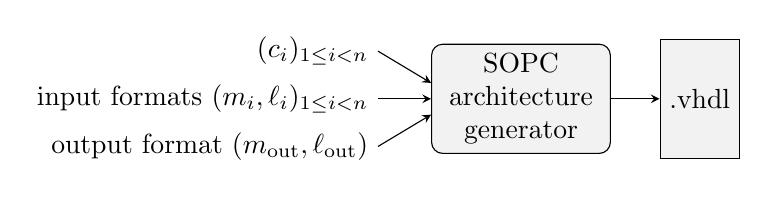
\begin{tikzpicture}
      \node[draw,align=center,fill=black!5,rounded corners, minimum width=15ex, minimum height=5ex] (flopoco) at (0,2ex) {
%$\displaystyle \sum_{i=0}^{n}c_ix_i $\\[1ex]
SOPC\\architecture\\generator};
      \node[left] (ai)      at (-12ex,6ex)  {$(c_i)_{1\le i < n}$};   
      \node[left] (precx)   at (-12ex,2ex) {input formats $(m_i, \ell_i)_{1\le i < n}$};   
      \node[left] (precy)   at (-12ex,-2ex) {output format $(m_\text{out}, \ell_\text{out})$};   
%      \node[] (target)  at (-7ex,-6ex) {FPGA};   
%      \node[] (freq)    at (3ex,-6ex)  {frequency};   
      \node[draw, rectangle,fill=black!5, minimum height=10ex] (vhdl) at (15ex,2ex) {.vhdl};   
      \draw[->,>=stealth] (ai.east) -- (flopoco.170) ;
      \draw[->,>=stealth] (precx.east) -- (flopoco.180) ;
      \draw[->,>=stealth] (precy.east) -- (flopoco.190) ;
%      \draw[->,>=stealth] (target) -- (flopoco.240) ; 
%      \draw[->,>=stealth] (freq) -- (flopoco.290) ;
      \draw[->,>=stealth] (flopoco.east) -- (vhdl.west) ;

      % \draw[dotted,black!50] (-34ex,-12ex) rectangle +(23ex,20ex);   
      % \node[black!50]  at (-23ex,-10ex) {\emph{Functional spec.}};   
      % \draw[dotted,black!50] (-10ex,-12ex) rectangle +(18ex,8ex);   
      % \node[black!50]  at (-1ex,-10ex) {\emph{Performance spec.}};   
  \end{tikzpicture}
  \caption{Interface to a sum-of-product-by-constant generator}
  \label{fig:interfaceSOPC}
\end{figure}

\subsection{Datapath analysis}


The fixed-point summation of the various terms $c_ix_i$ is depicted on Fig.~\ref{fig:maggraph1}.
For this figure, we take as an example a 4-input SOPC with arbitrary coefficients.
As shown on the figure, the exact  product of a real $c_i$ by an input $x_i$ may have an infinite number of bits. 

\subsubsection{Determining the most significant bit of $c_ix_i$ \label{sec:determ-most-sign}}
A first observation is that the MSB of the products $c_ix_i$ is completely determined by the $c_i$ and the input fixed-point format.
Indeed, we have fixed-point, hence bounded, inputs. 
If the domain of $x_i$ is $x_i\in (-1,1)$, the  MSB of $c_ix_i$ is the MSB of $|c_i|$.
This is illustrated by Figure \ref{fig:maggraph1}.
In general, if $|x_i|<M$, the MSB of $c_ix_i$ will be $\lceil \log_2(|c_i|M)\rceil$.

 
\begin{figure}
  \begin{boxedminipage}{\columnwidth}
  \centering
  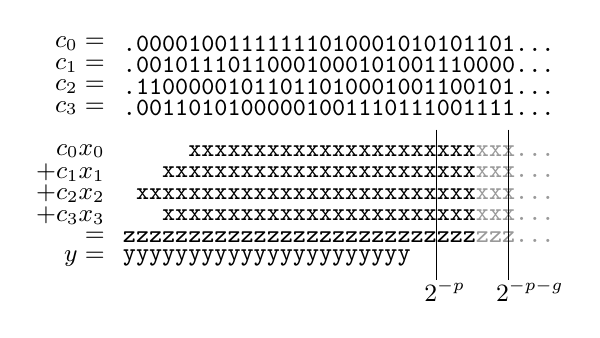
\begin{tikzpicture}
    \small 
    \draw
    (0ex, 10ex)     node[left] {$c_0 = $}  node[right,font=\tt] {.00001001111111010001010101101...}
    ++(0ex, -2ex)  node[left] {$c_1 = $}  node[right,font=\tt] {.00101110110001000101001110000...}
    ++(0ex, -2ex)  node[left] {$c_2 = $}  node[right,font=\tt] {.11000001011011010001001100101...}
    ++(0ex, -2ex)  node[left]  {$c_3 = $} node[right,font=\tt] {.00110101000001001110111001111...};
%  c_0 = 0.0195090...	
%  c_1 = 0.1826832... 		 =  .00101110110001000101001110000... 
%   c_2 = 0.7555706... 		 =  .11000001011011010001001100101...
%   c_3 = 0.2071065... 		 =  .00110101000001001110111001111...

   \draw  
   (0ex, 0ex)     node[left]  {$c_0x_0 $}  node[right,font=\tt] (xa0b) {~~~~~xxxxxxxxxxxxxxxxxxxxxx\textcolor{light-gray}{xxx...}}
   ++(0ex, -2ex)  node[left]  {$+c_1x_1 $}  node[right,font=\tt] (xa0b) {~~~xxxxxxxxxxxxxxxxxxxxxxxx\textcolor{light-gray}{xxx...}}
   ++(0ex, -2ex)  node[left]  {$+c_2x_2 $}  node[right,font=\tt] (xa0b) {~xxxxxxxxxxxxxxxxxxxxxxxxxx\textcolor{light-gray}{xxx...}}
   ++(0ex, -2ex)  node[left]  {$+c_3x_3 $}  node[right,font=\tt] (xa0b) {~~~xxxxxxxxxxxxxxxxxxxxxxxx\textcolor{light-gray}{xxx...}}
   ++(0ex, -2ex)  node[left]  {$ =  $}    node[right,font=\tt] (xa0b) {zzzzzzzzzzzzzzzzzzzzzzzzzzz\textcolor{light-gray}{zzz...}}
   ++(0ex, -2ex)  node[left]  {$y =  $}    node[right,font=\tt] (xa0b) {yyyyyyyyyyyyyyyyyyyyyy};
   \draw (30.1ex, 2ex) -- ++(0ex,-14ex) ++(-2ex,-1ex)  node[right]{$2^{-p}$};
   \draw (36.8ex, 2ex) -- ++(0ex,-14ex) ++(-2ex,-1ex) node[right]{$2^{-p-g}$};
%  c_0 = 0.0195090...	
%  c_1 = 0.1826832... 		 =  .00101110110001000101001110000... 
%   c_2 = 0.7555706... 		 =  .11000001011011010001001100101...
%   c_3 = 0.2071065... 		 =  .00110101000001001110111001111...
  \end{tikzpicture}
  \end{boxedminipage}
  \caption{The alignment of the $c_ix_i$ follows that of the $c_i$}
  \label{fig:maggraph1}
\end{figure}

This is obvious if  $c_ix_i$ is positive. 
It is not true if  $c_ix_i$ is negative, since in two's complement it needs to be sign-extended to the MSB of the result.
However  the sign extension of a signed number $\tt sxxxx$, where $\tt s$ is the sign bit, may be performed as follows \cite{ErcegovacLang2003}:
\begin{eqnarray}
  \label{eq:signext}
  \tt
   &&\tt 00...0\overline{s}xxxxxxx \nonumber\\[-1ex]
   &+ &\tt 11...110000000 \nonumber\\[-0.5ex]
   &= &\tt ss...ssxxxxxxx\nonumber
\end{eqnarray}

Here $\tt \overline{s}$ is the complement of $\tt s$. 
The reader may check this equation in the two cases, $\mathtt{s}=0$ and $\mathtt{s}=1$. 
Now the variable part of the product has the same MSB as $|c_i|$, just as in the positive case.

This transformation is not for free: we need to add a constant.
Fortunately, in the context of a summation, we may add in advance all these constants together.
Thus the overhead cost of two's complement in a summation is  limited to the addition of one single constant.
In many cases, as we will see, this addition can even be merged for free in the computations of the $c_ix_i$.


\subsubsection{Determining the least significant bit: error analysis for a sum of product \label{sec:erroranalysis}}
As we have seen, a single integer $p$,  the weight of the  least significant bit (LSB) of the output, also specifies  the accuracy of the computation. 

However, performing all the internal computations to this precision would not be accurate enough. 
Suppose for instance that we could build perfect hardware constant multipliers,  returning the perfect rounding $\widetilde{p}_i=\circ_p(c_ix_i)$ of the mathematical product $c_ix_i$ to precision $p$. 
Even such a perfect multiplier would entail an error, defined as $\abserr_i = \widetilde{p}_i - c_ix_i$, and bounded by $ \abserr_i < \maxerr_{\text{mult}}=2^{-p-1}$. 
Again this rounding error is the consequence of the limited-precision output format.
The problem is that in a SPC, such rounding errors add up.
Let us analyze this.

The output value $\widetilde{y}$ is computed in an architecture as the sum of the $\widetilde{p}_i$. 
This summation, as soon as it is performed with adders of the proper size, will entail no error.
Indeed, fixed-point addition of numbers of the same format may entail overflows (these have been taken care of above), but no rounding error.
This enables us to write 
\begin{eqnarray}
  \label{eq:errorlesssum}
  \widetilde{y}&=&\sum_{i=0}^{N-1} \widetilde{p}_i, 
 \end{eqnarray}

therefore 
\begin{eqnarray}
  \label{eq:globalerror}
  \abserr &= & \sum_{i=0}^{N-1} \widetilde{p}_i - \sum_{i=0}^{N-1} c_i x_i 
  \quad = \quad \sum_{i=0}^{N-1} \abserr_i \quad .
\end{eqnarray}

Unfortunately, in the worst case, the sum of the $\abserr_i$ can come close to $N\maxerr_{\text{mult}}$, which, as soon as $N>2$, is larger than $2^{-p}$:
this naive approach is not last-bit accurate.

The solution is, however, very simple. 
A slightly larger intermediate precision, with $g$ additional bits (``guard'' bits) may be used. 
The error of each multiplier is now bounded by $\maxerr_{\text{mult}}=2^{-p-1-g}$. 
It can be made arbitrarily small by increasing $g$.
Therefore, there exists some $g$ such that  $N\maxerr_{\text{mult}} <2^{-p-1}$
Actually, this is true even if a less-than-perfect multiplier architecture is used, as soon as we may compute a bound $\maxerr_{\text{mult}}$ of its accuracy,
and this bound is proportional to  $2^{-g}$. 

However, we now have another issue: the intermediate result now has $g$ more bits at its LSB than we need. 
It therefore needs itself to be rounded to the target format.
This is easy, using the identity $\circ(x)=\lfloor x+\frac{1}{2}\rfloor$:
rounding to precision  $2^{-p}$ is obtained by first adding $2^{-p-1}$ (this is a single bit) then discarding bits lower than $2^{-p}$.
However, in the worst case, this will entail an error $\abserr_{\text{final rounding}}$ of at most $2^{-p-1}$.

To sum up, the overall error of a faithful architecture SCP is therefore  
\begin{eqnarray}
  \label{eq:globalerrorfinal}
  \abserr &= & {\abserr_{\text{final rounding}}} + \sum_{i=0}^{N-1} \abserr_i 
  \quad <  \quad 2^{-p-1} + N\maxerr_{\text{mult}}
\end{eqnarray}
and this error can be made smaller than $2^{-p}$ as soon as we are able to build multipliers such that 
\begin{eqnarray}
  \label{eq:epsmultconstraint}
  N\maxerr_{\text{mult}} <2^{-p-1} \quad .
\end{eqnarray}







\subsection{LUT-based architectures computing just right for FPGAs}



All the previous was quite independent of the target technology: it could apply to ASIC synthesis as well as FPGA.
%Indeed, another team arrived to very similar conclusions roughly at the same time \cite{2014-HilaireLopezLSD-PECSS}.
Also, a very similar analysis can be developed for an inner-product architecture where the $c_i$ are not constant. 


The remainder of this section, conversely, is more focused on a particular context: LUT-based SCP architectures for FPGAs.
It explores architectural means to reach last-bit accuracy at the smallest possible cost (``computing just right'').

On most FPGAs, the basic logic element is the look-up-table (LUT), a small memory addressed by $\alpha$ bits. 
On the current generation of  FPGAs, $\alpha=6$.

\subsubsection{Perfectly rounded constant multipliers}
\label{sec:tabulatedmults}
As we have a finite number of possible values for $x_i$, it is possible to build a perfectly rounded multiplier by simply tabulating all the possible products.
The precomputation of table values must be performed with large enough accuracy (using multiple-precision software) to ensure the correct rounding of each entry.  
This even makes perfect sense for small input precisions on recent FPGAs:
if $x_i$ is a 6-bit number, each output bit of the perfectly rounded product $c_ix_i$  will consume exactly one 6-input LUTs.
For 8-bit inputs, each bit consumes only $4$ LUTs. 
In general, for $(6+k)$-bit inputs, each output bit consumes $2^k$ 6-LUTs: this approach scales poorly to larger inputs.
 However, perfect rounding to $p+g$ bits means a maximum error smaller than an half-LSB: 
 $\maxerr_{\text{mult}}  = 2^{-p-g-1}$.
Note that for real-valued $c_i$, this is more accurate than using a perfectly rounded multiplier that inputs  $\circ_p(c_i)$: 
this would accumulate two successive rounding errors.

\subsubsection{Table-based constant multipliers for FPGAs}
\label{sec:KCMmults}

\begin{figure}[b]
  \begin{center}
  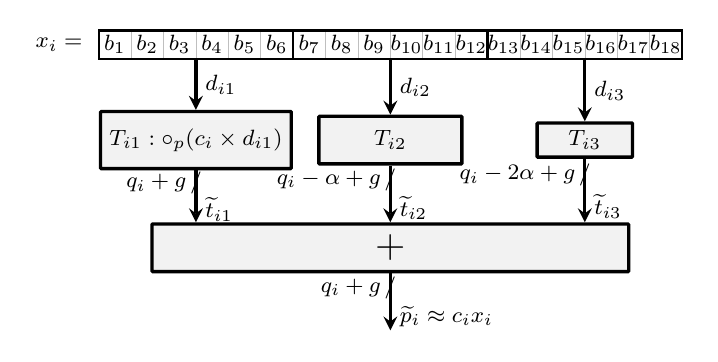
\begin{tikzpicture}
    \footnotesize 
    \node at (-1em,0)  {$x_i=$} ;
    \foreach \x in {1,...,18} {
%    \draw[] ($(-5*\x ex, -7ex)$) -- ($(-5*\x ex, -5ex)$) node[above] {$2^\x$} ;
      \node (n) at ($(3.4*\x ex, 0ex)$)  {$b_{\x}$} ;
      \draw[black!25, very thin] ($(n)+(1.7ex,1.5ex)$) -- ++(0, -3ex);
    }
    \node[draw, thick, rectangle, minimum width = 3.4*6ex, minimum height=3ex] (d1) at (3.4*3ex+1.7ex,0) {} ;
    \node[hwblock, minimum width=20ex,minimum height=6ex] (T1) at ($(d1)+(0,-10ex)$) { $T_{i1}: \circ_p(c_i\times d_{i1})$};
    \draw[hwbus,->] (d1.south) --  (T1.north) node[midway,right] {$d_{i1}$};

    \node[draw, thick, rectangle, minimum width = 3.4*6ex, minimum height=3ex] (d2) at (3.4*9ex+1.7ex,0) {} ;
    \node[hwblock, minimum width=15ex] (T2) at ($(d2)+(0,-10ex)$) { $T_{i2}$};
    \draw[hwbus,->] (d2.south) --  (T2.north) node[midway,right] {$d_{i2}$};

    \node[draw, thick, rectangle, minimum width = 3.4*6ex, minimum height=3ex] (d3) at (3.4*15ex+1.7ex,0) {} ;
    \node[hwblock, minimum width=10ex,minimum height=3.5ex] (T3) at ($(d3)+(0,-10ex)$) { $T_{i3}$};
    \draw[hwbus,->] (d3.south) --  (T3.north) node[midway,right] {$d_{i3}$};

    
    \node[hwblock, minimum width=50ex] (sum) at ($(T2)+(0,-11.3ex)$) {\Large $+$};
    \draw[hwbus,->]  (T1.south) --  ($(sum.80)!(T1)!(sum.north)$) % This means: point that is the projection of T1 on the line  (sum.80) -- (sum.north)
       node[near start] {$/$} node[near start,left] {$q_i+g$}          node[near end,right] {$\widetilde{t}_{i1}$};
    \draw[hwbus,->]  (T2.south) --  ($(sum.80)!(T2)!(sum.north)$) node[near start] {$/$} node[near start,left] {$q_i-\alpha+g$}   node[near end,right] {$\widetilde{t}_{i2}$};
    \draw[hwbus,->]  (T3.south) -- ($(sum.80)!(T3)!(sum.north)$) node[near start] {$/$} node[near start,left] {$q_i-2\alpha+g$}  node[near end,right] {$\widetilde{t}_{i3}$};

    \draw[hwbus,->] (sum.south) --  ++(0,-6ex) node[near start] {$/$} node[near start,left] {$q_i+g$} node[near end,right] {$\widetilde{p}_i\approx c_ix_i$};
 \end{tikzpicture}
\end{center}
\caption{The FixRealKCM method when $x_i$ is split in 3 chunks   \label{fig:FixRealKCM}}
\end{figure}

For larger precisions, we may use a variation of the KCM technique, due to Chapman  \cite{Chapman93:edn} and further studied by Wirthlin \cite{Wirthlin2004}.
The original KCM method addresses the multiplication by an integer constant.
We here present a variation that performs the multiplication by a \emph{real} constant.

This method  consists in breaking down the binary decomposition of an input $x_i$ into $n$ chunks $d_{ik}$ of $\alpha$ bits. 
With the input size being $m+f$,  we have $n=\lceil(m+f)/\alpha\rceil$ such chunks ($n=3$ on Figure~\ref{fig:FixRealKCM}). 
Mathematically, this is written
\begin{equation}
\displaystyle x_i\ =\ \sum_{k=1}^n 2^{-k\alpha}d_{ik}\quad \text{where}\quad d_{ik}\in\{0,...,2^\alpha-1\} \quad .
\label{eq:inputdec}
\end{equation}

The product becomes
\begin{equation}
\displaystyle c_ix_i\ =\ \sum_{k=1}^n 2^{-k\alpha} c_id_{ik} \quad .
\label{eq:KCM}
\end{equation}
Since each chunk $d_{ik}$ consists of $\alpha$ bits, where $\alpha$ is the LUT input size, we may tabulate each product $c_id_{ik}$ in a look-up table that will consume exactly one $\alpha$-bit LUT per output bit. 
This is depicted on Figure~\ref{fig:FixRealKCM}.
Of course, $c_id_{ik}$ has an infinite number of bit in the general case: as previously, we will round it to precision $2^{-p-g}$. 
In all the following, we define $\widetilde{t}_{ik}=\circ_p (c_id_{ik})$ this rounded value (see Figure~\ref{fig:KCMmaggraph}).

Contrary to classical (integer) KCM, all the tables do not consume the same amount of resources. 
The factor $2^{-k\alpha}$  in (\ref{eq:KCM}) shifts the MSB of the table output $\widetilde{t}_{ik}$, as illustrated by Figure~\ref{fig:KCMmaggraph}.


Here also, the fixed-point addition is errorless. 
The error of such a multiplier therefore is the sum of the errors of the $n$ tables, each perfectly rounded:  
\begin{equation}
\abserr_{\text{mult}} <n\times 2^{-p-g-1} \quad .
\label{eq:errorKCM}
\end{equation}

This error is proportional to $2^{-g}$, so can made as small as needed by increasing $g$.

\begin{figure}
  \begin{boxedminipage}{\columnwidth}
  \centering
  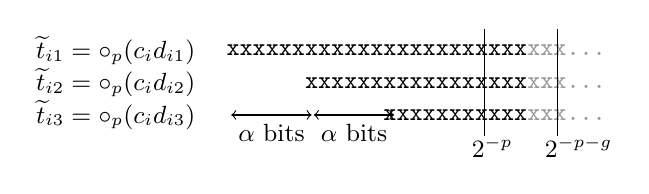
\begin{tikzpicture}
    \small 
   \draw  
   (0ex, 0ex)     node[left]  {$\widetilde{t}_{i1}=\circ_p (c_id_{i1})$}  node[right,font=\tt] (xa0b) {~xxxxxxxxxxxxxxxxxxxxxxx\textcolor{light-gray}{xxx...}}
   ++(0ex, -3ex)  node[left]  {$\widetilde{t}_{i2}=\circ_p (c_id_{i2})$}  node[right,font=\tt] (xa0b) {~~~~~~~xxxxxxxxxxxxxxxxx\textcolor{light-gray}{xxx...}}
   ++(0ex, -3ex)  node[left]  {$\widetilde{t}_{i3}=\circ_p (c_id_{i3})$}  node[right,font=\tt] (xa0b) {~~~~~~~~~~~~~xxxxxxxxxxx\textcolor{light-gray}{xxx...}}
   ;
   \draw (26.1ex, 2ex) -- ++(0ex,-10ex) ++(-2ex,-1ex)  node[right]{$2^{-p}$};
   \draw (32.9ex, 2ex) -- ++(0ex,-10ex) ++(-2ex,-1ex) node[right]{$2^{-p-g}$};

   \draw[<->] (10.2ex,-6ex) -- ++(7.5ex, 0) node [midway, below] {$\alpha$ bits};
   \draw[<->] (2.5ex,-6ex) -- ++(7.5ex, 0) node [midway, below] {$\alpha$ bits};
  \end{tikzpicture}
\end{boxedminipage}
  \caption{Aligment of the terms in the KCM method}
  \label{fig:KCMmaggraph}
\end{figure}



\subsubsection{Computing the sum}
In FPGAs, each bit of an adder also consumes one LUT.
Therefore, in a KCM architecture, the LUT cost of the summation is expected to be roughly proportional to that of the tables. 
However, this can be improved by stepping back and considering the summation at the SPC level.
Indeed, our faithful SPC result is now obtained by computing a double sum:
\begin{equation}
  \label{eq:SPCwithKCM}
  \widetilde{y}=\circ_p\left( \sum_{i=0}^{N-1}\sum_{k=1}^n 2^{-k\alpha} \widetilde{t}_{ik} \right)
\end{equation}
 
Using the associativity of fixed-point addition, this summation can be implemented very efficiently using compression techniques developed for multipliers \cite{ErcegovacLang2003} and more recently applied to sums of products \cite{parendeh2011:TRETS,2012-ICCD-Kumar-SOP}.
In FloPoCo, we may use the bit-heap framework introduced in  \cite{DinIstSer2013-FPL-BitHeap}.
Each table throws its $\widetilde{t}_{ik}$ to a bit-heap that is in charge of performing the final summation.
The bit-heap framework is naturally suited to adding terms with various MSBs, as is the case here.

This is illustrated on Fig.~\ref{fig:bitheaps}, which shows the bit heaps for two classical filters from \cite{ZigBeeStandard}.
On these figures, we have binary weights on the horizontal axis, and the various terms to add on the vertical axis.
These figure are generated by FloPoCo before bit heap compression.

We can see that the  shape of the bit heap reflects the various MSBs of the $c_i$. 
One bit heap is higher than the other one, although they add the same number of product and each product should be decomposed into the same number of KCM tables.
This is due to special coefficient values that lead to specific optimizations.
For instance $c_i=1$ or $c_i=0.5$ lead to a single addition of $x_i$ to the bit heap; $c_i=0$ leads to nothing.

\begin{figure}
  \begin{center}
    \begin{tabular}{cc}
    \includegraphics[width=0.45\columnwidth]{BitHeap_initial_hs} &
    \includegraphics[width=0.45\columnwidth]{BitHeap_initial_FixFIR_rrc}\\
    \footnotesize   Half-Sine &\footnotesize Root-Raised Cosine 
\end{tabular}
  \end{center}
  \caption{Bit heaps for two 8-tap, 12-bit FIR filters generated for Virtex-6}
  \label{fig:bitheaps}
\end{figure}

\subsubsection{Managing the constant bits}
Actually there are two more terms to add to the summation of Eq.~(\ref{eq:SPCwithKCM}): the rounding bit $2^{-p-1}$, necessary for the final rounding-by-truncation as explained in Section~\ref{sec:erroranalysis}, and the sum of all the sign-extension constants introduced in Section~\ref{sec:determ-most-sign}. These bits, especially the rounding bit, are visible on  Fig.~\ref{fig:bitheaps}.

There is a minor optimization to do here: these constant bits form a binary constant that can be added (at table-filling time) to all the values of one of the tables, for instance $T_{00}$.
Then the rounding bit will be added for free. 
The sign extension constants may add a few MSB bits to the table output, hence increase its cost by a few LUTs.
Still, with this trick, the summation to perform is  indeed given by Eq.~(\ref{eq:SPCwithKCM}), and the final rounding, being a simple truncation, is for free.
This optimization will be integrated to our implementation before publication.



Finally, the typical architecture generated by our tool is depicted by Figure~\ref{fig:Overall architecture}.

\begin{figure}
  \begin{center}
  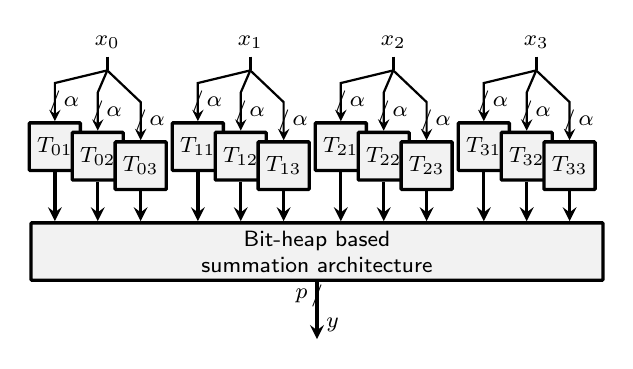
\begin{tikzpicture}
    \footnotesize 
    
    \node[hwblock, align=center,minimum width=60ex] (sum) at ($(32ex,-5ex)$) {Bit-heap based \\ summation architecture};

    \foreach \i in {0,...,3} {
      \node (x) at  ($(15*\i ex+10ex, 17ex)$) {$x_\i$};
      \coordinate (xb) at  ($(x)+(0, -3ex)$);
      \draw[hwbus,very thick] (x) --  (xb);
      
      \foreach \k in {1,...,3} {
        \node[hwblock, minimum width=5ex] (T) at ($(15*\i ex+4.5*\k ex,7ex-1*\k ex)$) { $T_{\i\k}$};
        \draw[hwbus,thick,<-]  (T.north) -- ++(0,+4ex) node [midway] {/}node [midway,right] {$\alpha$} -- (xb);
        \draw[hwbus,->] (T.south) --  ($(sum.north)!(T)!(sum.80)$);
      }
    }

    \draw[hwbus,->] (sum.south) --  ++(0,-6ex) node[near start] {$/$} node[near start,left] {$p$} node[near end,right] {$y$};
 \end{tikzpicture}
\end{center}
\caption{KCM-based SPC architecture for $N=4$, each input being split into 3 chunks  \label{fig:Overall architecture}}
\end{figure}





\section{Error analysis of direct-form  LTI filter implementations \label{sec:erroranalysisLTI}}
%\subsection{Definitions and abstract architecture }
This section shows how to obtain an implementation of the mathematical definition (\ref{eq:ideal-filter}) in fixed-point with last-bit accuracy on the computed result with respect to this  mathematical definition.
This computation is performed by the abstract architecture of Figure~\ref{fig:ltiarch}.

\begin{figure*}
  \centering
  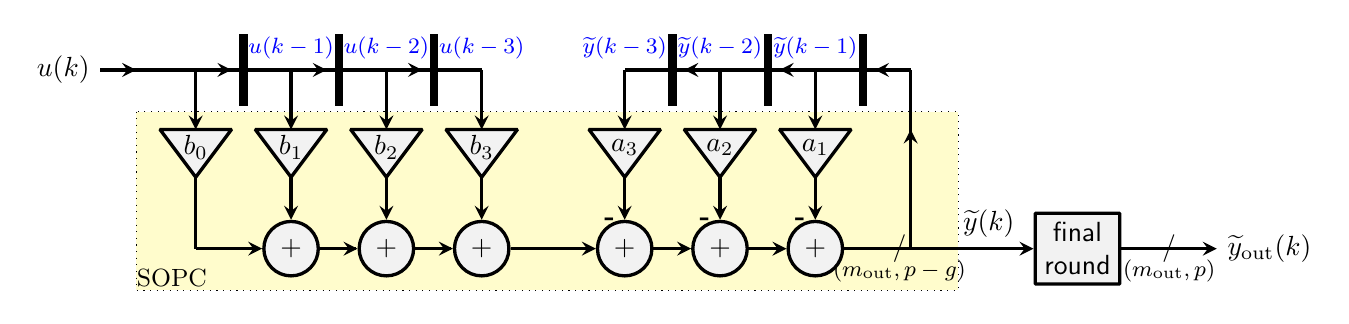
\begin{tikzpicture}
     \draw[dotted,black, fill=yellow!20] (-5ex,-3.5ex) rectangle +(69ex,-15ex);   
     \node[black]  at (-2ex,-17.5ex) {{\small SOPC}};   
    \draw[hwbus] (-8, 0) node[left] {$u(k)$} --  ++(8, 0)  ;
    \draw[hwbus,->] (-8, 0) --  ++(3, 0); % just for the arrow
    \foreach \i in {0,...,3} {
      \draw[hwbus, ->] ($(8*\i, 0)$) --  ++(0, -5);
      \draw[hwblock] ($(8*\i, -5)$) -- ++(3, 0) -- ++(-3, -4) -- ++(-3, 4) -- cycle; 
      \node (n) at ($(8*\i , -6.5)$)  {$b_{\i}$} ;
%      \draw ($(8*\i  + 0.5, -11)$) node[left,tt=black!50] {\footnotesize $p_b(k,\i)$} ;
%      \draw ($(8*\i  - 0.2, -11)$) node[right,text=black!50] {\footnotesize $p_b(k,\i)$} ;

%      \draw[hwbus, ->] ($(8*\i ex, 0ex)$) --  ++(0, -5ex);
    }

    
    \draw[hwbus] (0, -9) -- ++(0,-6);
      \coordinate (n) at  (0,-15);
    \foreach \i in {1,...,3} {
      \draw[line width=3pt] ($(8*\i  - 4, -3)$) --  +(0, 6);
      \draw[hwbus] ($(8*\i  - 8, 0)$) --  +(8,0) node [above,text=blue] {\footnotesize $u(k-\i)$};
      \draw[hwbus,->] ($(8*\i  - 8, 0)$) --  ++(3, 0); % just for the arrow
      % The adders 
      \coordinate (nm1) at  (n.east);
      \draw ($(8*\i , -15)$) node[hwblock,circle,minimum height=3] (n) {$+$};
      \draw[hwbus, ->]  ($(8*\i , -9)$) -- (n.north);
      \draw[hwbus, ->]  (nm1) -- (n.west);
      \draw[hwbus]  (n.east) -- ++ (3,0);
    }

    \draw (74, -15) node[hwblock,align=center] (fr) {final\\round} ;
    \draw[hwbus, <-] (fr.west) -- ++(-15,0) node [near end] {/} node [near end,below] {\footnotesize$(\msbout, p-g$)} node[near start,above] {$\appr{y}(k)$} -- ++(-1,0) ;
    \draw[hwbus, ->] (fr.east) -- ++(8,0) node [midway] {/} node [midway,below] {\footnotesize$(\msbout,p)$} node[right] {$\yout(k)$} ;

    \foreach \i in {1,...,3} {
      \draw[hwbus, ->] ($(-8*\i  + 60 , 0)$) --  ++(0, -5);
      \draw[hwblock] ($(-8*\i  + 60 , -5)$) -- ++(3, 0) -- ++(-3, -4) -- ++(-3, 4) -- cycle; 
      \node (ai) at ($(-8*\i  + 60 , -6.5)$)  {$a_{\i}$} ;
      %\draw ($(-8*\i  +60 + 0.5, -11)$) node[left,text=black!50] {\footnotesize $p_a(k,\i)$} ;
      %\draw ($(-8*\i  +60 - 0.2, -11)$) node[right,text=black!50] {\footnotesize $p_a(k,\i)$} ;
      \draw ($(-8*\i  + 60 , -15)$) node[hwblock,circle,minimum height=3] (n) {$+$};
      \draw (n.north) node[left]{\bf -};
      \draw[hwbus, ->] ($(-8*\i  + 60, -9)$) --  (n.north);
      \draw[hwbus, <-] (n.west) -- ++(-5,0);
      % The registers
      \draw[hwbus] ($(-8*\i  + 60  +8, 0)$) --  ++(-8, 0) node [above,text=blue] {\footnotesize $\appr{y}(k-\i)$};
      \draw[hwbus,->] ($(-8*\i  + 60  +8, 0)$) --  ++(-3, 0); % just for the arrow
      \draw[line width=3pt] ($(-8*\i  +60 + 4, -3)$) --  +(0, 6);
    }
    \draw[hwbus] ($(60 , 0)$) --  ++(0,-15);
    \draw[hwbus,<-] ($(60 , -5)$) --  ++(0,-5);


  \end{tikzpicture}

\caption{Abstract architecture for the direct form realization of an LTI filter \label{fig:ltiarch}}
\end{figure*}



The architecture of Figure~\ref{fig:ltiarch} computes an approximate value $\yout(k)$ that differs from  the idead value defined by  (\ref{eq:ideal-filter}) because of several occurences of discretization and rounding.
Formally, we refine the definition of the overall evaluation error as 
\begin{eqnarray}
  \epstotal(k)\ &= & \yout(k) - y(k)\label{eq:ltierr0}
\end{eqnarray}

Let us now decompose this error into its sources.


\subsection{Final rounding of the internal format} 

The architecture needs to internally use a fixed-point format that offers extended precision with respect to the input/output format.
From another point of view, this internal format offers $g$ additional LSB bits (usually called \emph{guard bits}) in which rounding errors may accumulate without touching the output bits. 
The sequel will show more formally how to compute an optimal value of this architectural parameter $g$. 
Anyway we need to round the internal result from this extended format to the output format (in the ``final round'' box on Figure~\ref{fig:ltiarch}). 
This entails an additional error $\epsfinalround$, formally defined as 
\begin{equation}
  \label{eq:epsfinalround}
  \epsfinalround(k) = \yout(k) - \appr{y}(k)\quad.
\end{equation}
This error may be bounded by  $\maxepsfinalround = 2^{p-1}$ (round to nearest). 

Remark that we feed back the internal result $\appr{y}(k)$, not the output result $\yout(k)$. 
This  prevents an amplification of $\epsfinalround(k)$ by the feedback loop that could compromise the goal of faithful rounding. 

\subsection{Rounding and quantization errors in the sum of products} 

As the coefficients $a_i$ and $b_i$ are real numbers, they must be rounded to some finite value (quantization)  before the multiplication can take place. 
Then, the multiplication and the summation may themselves involve rounding errors.
Managing all these rounding errors will be the subject of section~\ref{sec:SoPC}, which will show how to build an architecture that achieves a given accuracy goal at the minimum cost. 
For now, we may summarize all these errors in a single term $\epssopc(k)$ mathematically defined as
\begin{eqnarray}
  \epssopc(k) &= & \appr{y}(k) -  \left(\sum_{i=0}^n b_iu(k-i) -\sum_{i=1}^n a_i\appr{y}(k-i)\right)
 \label{eq:epssopc}
\end{eqnarray}
This equation should be read as follows: $\epssopc(k)$ measures how much a result $\appr{y}(k)$ computed by the SOPC architecture diverges  from that computed by an ideal SOPC (that would use the infinitely accurate coefficients $a_i$ and $b_i$,  and be free of rounding  errors), this ideal SOPC being applied on the same inputs $u(k-i)$  and $\appr{y}(k-i)$ as the architecture.


\subsection{Error amplfication in the feedback loop}
 The input signal $u(k)$ can be considered exact, in the sense that whatever error it may carry is not due to the filter under consideration. 
However, the feedback signal $\appr{y}(k)$ that is input to the computation differs from the ideal $y(k)$. Let us now define $\epsytilde(k)$ as the error of $\appr{y}(k)$ with respect to $y(k)$:
\begin{eqnarray}
  \epsytilde(k)\ &= & \appr{y}(k) - y(k) .
 \label{eq:epsytilde}
\end{eqnarray}
This error is potentially amplified by the architecture.






Using  (\ref{eq:epsytilde}), let us  rewrite $\appr{y}(k-i)$ in  the right-hand side of (\ref{eq:epssopc}): 
\begin{eqnarray}
% tient pas sur une colonne
%  \epssopc(k)\ &= & \appr{y}(k) -  \left(\sum_{i=0}^n b_iu(k-i) -\sum_{i=1}^n a_i y(k-i) -\sum_{i=1}^n a_i \epsytilde(k-i) \right)  \label{eq:ltierr2} \\
  \epssopc(k)\ &= & \appr{y}(k) - \sum_{i=0}^n b_iu(k-i) +\sum_{i=1}^n a_i y(k-i) \nonumber \\
&&\quad + \sum_{i=1}^n a_i\epsytilde(k-i)  \label{eq:ltierr2} \nonumber\\
  &=& \appr{y}(k) -  y(k)  + \sum_{i=1}^n a_i \epsytilde(k-i) \quad \text{using (\ref{eq:ideal-filter})} \nonumber\\
  &=&\epsytilde(k) + \sum_{i=1}^n a_i \epsytilde(k-i) \quad \quad \text{using (\ref{eq:epsytilde})}.
  \label{eq:ltierr3}
\end{eqnarray}

If we rewrite (\ref{eq:ltierr3}) as 
\begin{eqnarray}
  \epsytilde(k)   &=& \epssopc(k) -  \sum_{i=1}^n a_i \epsytilde(k-i)
  \label{eq:ltierr4}
\end{eqnarray}
we obtain the equation of an LTI filter inputting $\epssopc(k)$ and outputting $\epsytilde(k)$, whose transfer function is 
\begin{equation}
  \label{eq:transferfun}
  \mathcal{H}_{\abserr}(z)=\frac{1}{1+\sum_{i=1}^{n}a_iz^{-i}}   \ .
\end{equation}

Finally, (\ref{eq:epsytilde}) can be rewritten
\begin{eqnarray}
 \appr{y}(k)  &= & y(k) +  \epsytilde(k) \label{eq:ltierrfinal}
\end{eqnarray}
which is illustrated by Figure~\ref{fig:ltierror}.

\begin{figure}[h] 
  \centering
  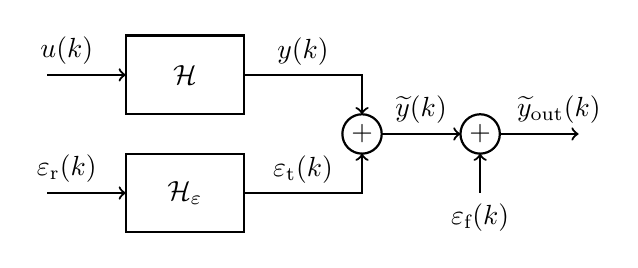
\begin{tikzpicture}[x=1cm,y=1cm]
    \draw (-2,0.5) rectangle ++(1.5,1)[thick] node [midway]{$\mathcal{H}$}; 
    \draw (-3, 1) -- (-2,1) [->, thick] node [above,near start]{$u(k)$}; 
    \draw (-0.5, 1)  -- (1,1) -- (1,0.5) [->, thick] node[xshift=-0.75cm,yshift=0.8cm]{$y(k)$}; 

    \draw (-2,-1) rectangle ++(1.5,1)[thick] node [midway]{$\mathcal{H}_{\abserr}$}; 
    \draw (-3, -0.5) -- (-2,-0.5) [->, thick] node[above,near start]{$\epssopc(k)$};
    \draw (-0.5, -0.5) -- (1,-0.5) -- (1,0) [->, thick] node [xshift=-0.75cm,yshift=-0.2cm]{$\epsytilde(k)$}; 

    \draw (1,0.25) circle (0.25) [thick] node {$+$}; 
    \draw (1.25,0.25) -- (2.25,0.25)[->, thick] node [above,midway] {$\appr{y}(k)$};

    \draw (2.5,0.25) circle (0.25) [thick] node {$+$}; 
    \draw (2.75,0.25) -- ++(1,0)[->, thick] node [above,near end] {$\yout(k)$};
    \draw (2.5,0) -- ++(0,-0.5)[<-, thick] node [below] {$\epsfinalround(k)$};
  \end{tikzpicture}

\caption{A signal view of the error propagation with respect to the ideal filter \label{fig:ltierror}}
\end{figure}


We can now apply Lemma~\ref{lemma:wcpg} to  $\mathcal{H}_{\abserr}$ with input $\epssopc$ in order to bound $\epsytilde$ by

\begin{eqnarray}
 \maxepsytilde& =& \wcpgHe \maxepssopc \ .
\end{eqnarray}

Therefore, we can also keep $\maxepsytilde$  as low as needed by increasing the internal precision to reduce $\maxepssopc$.


\subsection{Putting it all together}

We may now rewrite (\ref{eq:ltierr0}) as
\begin{eqnarray}
  \epstotal(k)\ &= & \yout(k) -\appr{y}(k) + \appr{y}(k) - y(k) \nonumber \\
  &=& \epsfinalround(k)+ \epsytilde(k)  \label{eq:ltierr16}
\end{eqnarray}

hence
\begin{eqnarray}
  \maxepstotal\ &= & \maxepsfinalround(k)+ \maxepsytilde \nonumber \\ 
 &=&  \maxepsfinalround(k)+ \wcpgHe \maxepssopc \label{eq:ltierr18}
\end{eqnarray}



The accuracy target for faithful rounding is $\maxepstotal=2^p$.
The final rounding implies an error bounded by $\maxepsfinalround=2^{p-1}$
To achieve faithful rounding, it therefore suffices that the error $\maxepsytilde$ of the filter before final rounding is bounded by $2^{-p-1}$.
This leads to the following constraint on $\maxepssopc$:
\begin{equation}
  \label{eq:erroramplificationcomp}
  \maxepssopc < \frac{2^{p-1}}{\wcpgHe} \quad.
\end{equation}

This constraint finally translates to the LSB $p-g$ of the intermediate result as follows.
Assuming we build an SOPC faithful to $p-g$, we will have $\maxepssopc<2^{p-g}$. 
Therefore the smallest number of guard bits ensuring that the constraint (\ref{eq:erroramplificationcomp}) holds is
\begin{equation}
  \label{eq:gfory}
  g= 1 + \lceil  \log_2\wcpgHe\rceil \quad.
\end{equation}



Meanwhile, the MSB of the intermediate format (which is the same as that of the result)  is completely determined by the constants:

\begin{equation}
%\text{MSB}_{\widetilde{y}} = \left\lceil \log_2(\sum_{i=0}^{N-1}|c_i|M)\right\rceil\ .\label{eq:MSBresult}
m_{\text{out}} = \left\lceil \log_2\wcpg{\mathcal{H}}\right\rceil\ .\label{eq:MSBresult}
\end{equation}

Some overflows may occur in the internal computation. 
However in which case the computation is performed modulo $2^{m_{\text{out}}}$, and the result will be correct.

% From (\ref{eq:overallltierror1}), this error is the sum of $n+m$ product rounding error. 
% If each of these is bounded by $\maxerr_{\text{mult}}$, it suffice to build Figure~\ref{fig:ltiarch} with multipliers such that 

% \begin{equation}
%   \label{eq:finalerrmultconstraint}
%   \maxerr_{\text{mult}} < \frac{2^{-p-1}}{(n+m)\wcpgHe} \quad.
% \end{equation}














\section{Implementation and results}

The method described in this paper is implemented as the \texttt{FixFIR} operator of FloPoCo. 
\texttt{FixFIR} offers the interface shown on Fig.~\ref{fig:interface}, and inputs the $c_i$ as arbitrary-precision numbers.
On top of it, the operators \texttt{FixHS} and \texttt{FixRRCF} simply evaluate the $c_i$ using the textbook formula for Half-Sine and Root-Raised Cosine respectively,  and feed them to \texttt{FixFIR}.  
We expect many more such wrappers could be written in the future.

\texttt{FixFIR}, like most FloPoCo operators, was designed with a testbench generator \cite{DinechinPasca2011-DaT}. 
All these operators reported here have been checked for last-bit accuracy by extensive simulation.

Table~\ref{tab:results:} reports synthesis results for architectures generated by \texttt{FixRRCF}, as of  FloPoCo SVN revision 2666. 
All the results were obtained for Virtex-6 (6vhx380tff1923-3)   using ISE 14.7.
These results are expected to  improve in the future, as the (still new) bit-heap framework is tuned in FloPoCo.  

\begin{table}
  \begin{center}
      \begin{tabular}{|c|c||c|cc|}
        \hline
        Taps		& I/O size &  Speed  		   	&      \multicolumn{2}{|c|}{Area} 	 \\
        \hline\hline
        \multirow{2}{*}{8} & \multirow{2}{*}{12 bits} &  4.4 ns (227 Mhz) & 564 LUT & \\
        &  &  1 cycle @ 344 Mhz & 594 LUT & 32 Reg.\\
        \hline
        \hline

        \multirow{2}{*}{8} & \multirow{2}{*}{18 bits} & 5.43ns (184 MHz) & 1325 LUT & \\
        &  & 2 cycles @ 318 MHz & 1342 LUT & 92Reg.\\
        \hline
        \hline

        \multirow{2}{*}{16} & \multirow{2}{*}{12 bits} &  5.8 ns (172 Mhz) & 1261 LUT & \\
        &  &  1 cycle @ 289 Mhz & 1257 LUT & 41 Reg.\\
        \hline
        \hline

        \multirow{2}{*}{16} & \multirow{2}{*}{18 bits} & 7.3 ns (137 MHz) & 2863 LUT &\\
        & &  2 cycles @ 265 MHz & 2810 LUT & 120 Reg.\\
        \hline
        % \hline
        % \multicolumn{5}{|c|}{Root-Raised Cosine}\\
        % \hline
        % \multicolumn{5}{|c|}{Half-sine}\\
        % \hline
        % 8 & 12 & 4.4 ns (215 Mhz) & 446 LUT & \\
        % & & 1 cycle @ 368 Mhz & 523 LUT & 29 Reg.\\
      \end{tabular}
      ~\\[0.5ex]
      Note: the register count does not include the input shift register. 
  \end{center}
  \caption{Synthesis results of a Root-Raised Cosine FIR.\label{tab:results:}}
\end{table}

\subsection{Analysis of the results}
As expected, the dependency of the area to the number of taps is almost linear. 
On the one hand, more taps increase the number of needed guard bits.
On the other hand, more taps mean a larger bit heap which exposes more opportunities for efficient compression. 
However, there is also the dependency of the $c_i$ themselves to the number of taps.

Conversely, the dependency of area on precision is more than linear. 
It is actually expected to be almost quadratic, as can be observed by evaluating the number of bits tabulated for each multiplier (see Fig.~\ref{fig:KCMmaggraph}).

Interestingly, the dependency of the delay to the number of taps is clearly sub-linear.
This is obvious from Fig.~\ref{fig:Overall architecture}. 
All the table accesses are performed in parallel, and the delay is dominated by the compression delay, which is logarithmic in the bit-heap height \cite{Dadda1965}.


\subsection{Comparison to a naive approach}

In order to evaluate the cost of computing just right, we built a variant of the \texttt{FixFIR} operator following a more classical approach.
In this variant, we first quantize all the coefficients to precision $p$ (\emph{i.e} such that their LSB has weight $2^{-p}$).
We obtain fixed-point constants, and we then build an architecture that multiplies these constants with the inputs using the classical (integer) KCM algorithm.

A simple error analysis shows that the mere quantization to precision $p$ is already responsible for the loss of two bits of accuracy on $\widetilde{y}$. 
The exact error due to coefficient quantization depends on the coefficients themselves but space is missing here to detail that.
Then, the multiplications are exact. 
However, as illustrated by Figure \ref{fig:intKCMmaggraph}, their exact results extend well below precision $2^p$: they have to be rounded.
We just truncate the output of each KCM operators to  $2^{-p}$.
This more than doubles the overall error. 
It also allows the synthesis tools to optimize out the rightmost 6 bits of Fig.~\ref{fig:intKCMmaggraph}.
Then these truncated products are summed using a sequence of $N-1$ adders of precision $p$.

The results are visible in Table~\ref{tab:results:cmp}. 
The naive approach leads to a much smaller, but slower design. 
The area difference doesn't come from the tables, if we compare Fig.~\ref{fig:KCMmaggraph} and Fig.~\ref{fig:intKCMmaggraph}. 
It comes from the summation, which is performed on $g$ more bits in the last-bit accurate approach.
Besides, only the last-bit accurate approach uses a bit heap, whose compression heuristics are currently optimized for speed more than for area.

However, this comparison is essentially meaningless, since the two architectures are not functionally equivalent: 
The proposed approach is accurate to 12 bits, while the naive approach loses more than 3 bits to quantization and truncation.
Therefore, a meaningful comparison is the proposed approach, but accurate to $p=9$, which we also show in Table~\ref{tab:results:cmp}. 
This version is better than the naive one in both area and speed.

Since we are comparing two designs by ourselves, it is always possible to dispute that we deliberately sabotaged our naive version. 
And in a sense, we did:
We designed it as small as possible (no guard bits, truncation instead of rounding, etc).
Short of designing a filter that returns always zero (very poor accuracy, but very cheap indeed), this is the best we can do. 
But all these choices are highly disputable, in particular because they impact accuracy.
  
All this merely illustrates the point we want to make: 
it only makes sense to compare designs of equivalent accuracies. 
And the only accuracy that makes sense is last-bit accuracy, for the reasons exposed in \ref{sec:LBA4ASAP}.  
We indeed put our best effort in designing the last-bit accurate solution, and we indeed looked for the most economical way of achieving a given accuracy. 
This is comforted by this comparison. 
Focussing on last bit accuracy enables us to compute right, and just right.

\begin{figure}
  \begin{boxedminipage}{\columnwidth}
  \centering
  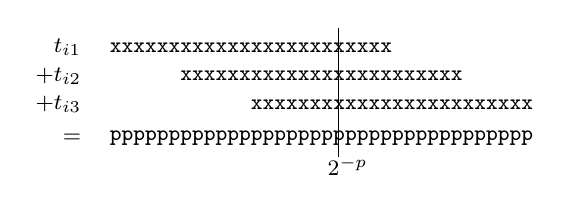
\begin{tikzpicture}
    \footnotesize
   \draw  
   (0ex, 0ex)     node[left]  {${t}_{i1}$}   node[right,font=\tt] (xa0b) {~xxxxxxxxxxxxxxxxxxxxxxxx}
   ++(0ex, -3ex)  node[left]  {$+{t}_{i2}$}  node[right,font=\tt] (xa0b) {~~~~~~~xxxxxxxxxxxxxxxxxxxxxxxx}
   ++(0ex, -3ex)  node[left]  {$+{t}_{i3}$}  node[right,font=\tt] (xa0b) {~~~~~~~~~~~~~xxxxxxxxxxxxxxxxxxxxxxxx}
   ++(0ex, -3.5ex) node[left]  {$=$}  node[right,font=\tt] (xa0b)       {~pppppppppppppppppppppppppppppppppppp}
   ;
   \draw (26.1ex, 2ex) -- ++(0ex,-13.5ex) ++(-2ex,-1ex)  node[right]{$2^{-p}$};

  % \draw[<->] (10.2ex,-6ex) -- ++(7.5ex, 0) node [midway, below] {$\alpha$ bits};
  % \draw[<->] (2.5ex,-6ex) -- ++(7.5ex, 0) node [midway, below] {$\alpha$ bits};
  \end{tikzpicture}
\end{boxedminipage}
  \caption{Using integer KCM: $t_{ik}=\circ_p (c_i)\times d_{ik}$. This multiplier   is both wasteful, and not accurate enough.}
  \label{fig:intKCMmaggraph}
\end{figure}
% \subsection{Comparison to DSP-based architectures}
For the sake of completeness, we also implemented a version  using DSP blocks, reported in Table \ref{tab:results:cmp}.
Considering the large internal precision of DSP blocks, it costs close to nothing to design this version as last-bit accurate for $p=12$ or $p=18$ (in the latter case, provided the constant is input with enough guard bits on the 24-bit input of the DSP block). This is very preliminary work, however. We should offer the choice between either an adder tree with a shorter delay, or a long DSP chain which would be slow, but consume no LUT. We should also compare to Xilinx CoreGen FIR compiler, which generates only DSP-based architectures.
Interestingly, this tool requires the user to quantize the coefficients and to take all sorts of decisions about the intermediate accuracies and rounding modes. 

\begin{table}
  \begin{center}
      \begin{tabular}{|l||c|c|c|}
        \hline
        Method                       &  Speed  		   	&      \multicolumn{1}{|c|}{Area}  & accuracy	 \\
        \hline
        \hline
         $p=12$, proposed &  4.4 ns (227 Mhz) & 564 LUT &  $\maxerr<2^{-12}$\\
        \hline
        $p=12$, naive &  5.9 ns (170 Mhz) & 444 LUT & $\maxerr>2^{-9}$\\
        \hline
        $p=9$, proposed &  4.12 ns (243 Mhz) & 380 LUT & $\maxerr<2^{-9}$\\
        \hline
        \hline
        $p=12$, DSP-based  &  9.1 ns (110 Mhz) & 153 LUT, 7 DSP  & $\maxerr<2^{-9}$\\
        \hline
      \end{tabular}
  \end{center}
  \caption{The accuracy/performance trade-off on 8-tap, 12 bit  Root-Raised Cosine FIR filters.\label{tab:results:cmp}}
\end{table}

% \subsection{Comparison with other works}
% %We are aware that this article misses 

% It is difficult to compare to other tools which have much more complex specifications. 
% For instance, the Xilinx CoreGen FIR compiler requires us to quantize the coefficients and to take all sorts of decisions about the intermediate accuracies and rounding modes. 
% %However, the main reason why we didn't attempt to compare to it is that it will generate only DSP-based architectures, while our approach is essentially LUT based.








~\\


\section*{Conclusion}

This paper claims that  sum-of-product architectures should be last bit accurate, and demonstrates that this has two positive consequences:
It gives a much clearer view on the trade-off between accuracy and performance, freeing the designer from several difficult choices.
It actually leads to better solutions by enabling a ``computing just right'' philosophy.
All this is demonstrated on an actual open-source tool that offers the highest-level interface.


Future work include several technical improvements to the current implementation, such as the exploitation of symmetries in the coefficients or optimization of the bit heap compression.

Beyond that, this work opens many perspectives.

 As we have seen, fixed-point sum of products and sum of squares could be optimized for last-bit accuracy using the same approach.  

 We have only studied one small corner of the vast literature about  filter architecture design. 
Many other successful approaches exist, in particular those based on multiple constant multiplication (MCM) using the transpose form (where the registers are on the output path)
\cite{Potkonjak94,BouTis2005:IEEETC,Mehendale95,VoronenkoPuschel2007,AskoyEtAl:2008}. 
A technique called Distributed Arithmetic, which predates FPGA \cite{White1989:DA}, can  be considered  a  generalization of the KCM technique to the MCM problem. 
From the abstract of \cite{2013-ReCoSoc-Kumm-DAvsKCM} that, among other things, compares these two approaches,  ``if the input word size is greater than approximately half the number of coefficients, the LUT based multiplication scheme needs less resources than the DA architecture and vice versa''. 
Such a rule of thumb (which of course  depends on the coefficients themselves) should be reassessed with architectures computing just right on each side.
Most of this vast literature treats  accuracy after the fact,  as an issue orthogonal to architecture design.

A repository of FIR benchmarks exists, precisely for the purpose of comparing FIR implementations \cite{FirSuite}. 
Unfortunately, the coefficients there are already quantized, which prevents a meaningful comparison with our approach.
Few of the publications they mention report accuracy results.
However, cooperation with this group should be sought to improve on this.


 We have only considered here the implementation of a filter once the $c_i$ are given. 
  Approximation algorithms, such as Parks-McClellan, that compute these coefficients, essentially work in the real domain. 
  The question they answer is ``what is the best filter with real coefficients that matches this specification''.
  It is legitimate to wonder if asking the question: ``what is the best filter with low-precision coefficients''  could not lead to a better result.

 Still in filter design, the approach presented here should be extended to  infinite impulse response (IIR) filters. 
  There, a simple worst-case analysis (as we did for SPC) doesn't work  due to the infinite accumulation of error terms. 
  However, as soon as the filter is stable (i.e. its output doesn't diverge), it is possible to derive a bound on the accumulation of rounding errors \cite{2012-HilaireLopezLSD-DASIP}.
  This would be enough to design last-bit accurate IIR filters computing just right.
%%%%%%%%%%%%%%%%%%%%%%%%%%%%%%%%%%%%%%%%%%%%%%%%%%%%%%%%%%%%%%%%%%%%%
\newpage

\bibliographystyle{IEEEtran}

% Florent dit: J'ai juste découvert bibexport ou esc X reftex-create-bibtex-file
% Chez moi j'utilise tout mon bordel de fichiers bib centralisés
%\bibliography{/home/fdedinec/Boulot/biblio/arenaire,/home/fdedinec/Boulot/biblio/arith,/home/fdedinec/Boulot/biblio/fpga,/home/fdedinec/Boulot/biblio/other,/home/fdedinec/Boulot/biblio/f2d}

% Mais si vous vous voulez que cela compile vous pouvez commenter cette ligne et la remplacer par la ligne suivante: 
\bibliography{biblio}


%Le fichier biblio.bib est extrait de mes bib par
%   bibexport -o biblio.bib FiltersCJR.aux
% ou esc X reftex-create-bibtex-file

% Si vous voulez ajouter des refs qui n'y sont pas mais que vous avez en local, vous pouvez faire comme moi...

% De mon coté si je vois apparaitre des refs dans le biblio.bib je les ajouterai à mes bibs centralisés 
\end{document}







